\documentclass[10pt,a4paper]{article}
\usepackage[]{algorithm2e}
\usepackage{amsfonts}
\usepackage{amsmath}
\usepackage{amssymb}
\usepackage[english]{babel}
\usepackage{caption}
\usepackage{enumitem}
\usepackage{float}
\usepackage[left=2cm,right=2cm,top=2cm,bottom=2cm]{geometry}
\usepackage{graphicx}
\usepackage[utf8]{inputenc}
\usepackage{pdfpages}
\usepackage{physics}
\usepackage{subcaption}
\usepackage{verbatim}

%%%%%%%%%%%%%%%%%%%%%%
% I didn't want to include a bibtex file since the project specifications didn't call for one
% from https://tex.stackexchange.com/questions/60649/using-bibtex-entries-directly-in-tex-file
\usepackage{amsrefs}
\newenvironment{rezabib}
  {\bibdiv\biblist\setupbib}
  {\endbiblist\endbibdiv}
  \def\setupbib{\catcode`@=\active}
\begingroup\lccode`~=`@
  \lowercase{\endgroup\def~}#1#{\gatherkey{#1}}
\def\gatherkey#1#2{\gatherkeyaux{#1}#2\gatherkeyaux}
\def\gatherkeyaux#1#2,#3\gatherkeyaux{\bib{#2}{#1}{#3}}
%%%%%%%%%%%%%%%%%%%%%%%

\title{CME 211 Project: Part 2}
\author{Joshua Barnett}
\begin{document}

\maketitle
\section*{Introduction}
The goal of the project is to create an OOP code that can solve the heat equation on a specific geometry under specified boundary conditions and the specifications are provided in [2]. This requires creating a sparse matrix class to form our block  diagonal system in a efficient CSR format suitable for a conjugate gradient method to solve the system $A x = b$. Finally, we save these results and process and visualize with a python script.
\section*{Description}
\subsection*{Conjugate Gradient method}
The conjugate gradient (CG) method for solving the linear system $A x = b$ requires a few matrix and vector operations that can be generalized into a few operations and is fully specified in \cite{Part1}. The most important function is a General Matrix Multiply (GEMM) that takes the form $c = \alpha A x + \beta b $ where $c$, $x$, and $b$ are vectors, $\alpha$ and $\beta$ are scalars, and $A$ is a CSR matrix. We can use this function for all of the matrix multiplication operations required in the CG method. Additionally, we also implement a weighted vector sum called daxby which is the expression $d = \alpha x + \beta y$. Finally, we have simple operations where we calculate the dot product and $L_2$ norm. These form the basis for all of the basic operations required to perform the CG method whose pseudo-code is defined below.

\begin{algorithm}
\KwData{Matrix $A$ and vector $b$ to solve $A x = b$}
 \KwResult{Solution for vector $x$ in $A x = b$ }
 $u_n = \mathbf{1}$\;
 $r_n = b - A u_n$\;
 $l_{2,0} = \text{norm}_2(r_n)$\;
 $p_n = r_n$\;
 $n = 0$\;
 \While{$ n < n_{max}$}{
  $n$\texttt{++}\;
  $\alpha = r_n^T r_n / \left(p_n^T A p_n\right)$\;
  $u_{n + 1} = u_n + \alpha p_n$\;
  $r_{n + 1} = r_n - \alpha A p_n$\;
  $l_{2,r} = \text{norm}_2\left(r_{n + 1}\right)$\;
  \If{$l_{2,r}/l_{2,0} < $ \texttt{tol}}{
   break\;
   }
  $\beta = r_{n+1}^T r_{n+1} /(r_n^T r_n)$\;
  $p_n = r_{n + 1} + \beta p_n$\;
  $u_n = u_{n + 1}$\;
  $r_n = r_{n + 1}$\;
 }
 \caption{Conjugate Gradient Method for solving $A x = b$}
\end{algorithm}

In order to facilate an OOP design, a few changes were made from the original code. Most importantly, the GEMM operation was altered to accept a new class called \texttt{SparseMatrix} instead of the list of \texttt{vector} objects.

\subsection*{\texttt{SparseMatrix} Design}
The \texttt{SparseMatrix} class is broken down into three \texttt{vector} objects containing \texttt{int}, \texttt{int}, and \texttt{double} respectively as well as two \texttt{int} members to hold the size of the matrix and finally a \texttt{bool} value to specify if the matrix is in CSR format or not. There a few methods implemented, including \texttt{Resize} which checks to make sure the new matrix sizes are compatible with current data. The \texttt{AddEntry} method ensures that the matrix is not already in CSR format before adding. The \texttt{ConvertToCSR} method simply calls the \texttt{COO2CSR} method and sets the \texttt{bool} for if it is CSR to \texttt{true}. In order to use the original GEMM method, a new method \texttt{CSR\_GEMM} is defined as a \texttt{friend} of the \texttt{SparseMatrix} class so it can access the private members when calling the original GEMM method.

\subsection*{\texttt{HeatEquation} Design}
The \texttt{HeatEquation} class contains the \texttt{SparseMatrix} defining the system of equations to solve $A x = b$ as well as a few \texttt{vector} objects of type \texttt{double} to hold the RHS and proposed solution vector. There are two public methods, \texttt{Setup} and \texttt{Solve} that perform the basic operations of the class. \texttt{Setup} loads data from the provided input file and creates the sparse matrix $A$ and vector $b$. The \texttt{Solve} class solves the system by calling the private function \texttt{CGIterate} which is copied from the \texttt{CGSolver} file inside the while-loop that way we have access to each iteration. It is too cumbersome to reuse the \texttt{CGSolver} method alone since it only provides the final answer and no intermediate results (like the $r$ and $p$ vectors).
\newline
The matrix we create unrolls the 2D grid of points into a linear vector as the variable $x$. Each gridpoint in general will depend on five points total: the gridpoint itself, one to the left and right, and one up and down. This is encapsulated in the discretization of the heat equation given in \cite{Part2}
$$ \frac{1}{h^2} \left(u_{i+1,j} + u_{i-1,j} + u_{i,j+1} + u_{i,j-1} - 4u_{i,j}\right) = 0 .$$
Thankfully, in constructing the matrix, we can simply add an entry for each term for the single point. This results in a banded sparse matrix. The boundary conditions are statisfied by only evaluating one side along the periodic boundary and otherwise only evaluating interior points (not on the isothermal boundaries). When a gridpoint references a boundary point, the value is instead added to the $b$ vector when solving $A x = b$ in the CG method.
\section*{User Guide}
\subsection*{Compiling the \texttt{C++} code}
After pulling the entire \texttt{project} directory, perform the following command:
\begin{verbatim}
$ [cd to project directory]
$ make
\end{verbatim}
This will produce a \texttt{main} executable that we can use to product a solution given an input file and prefix. The input file has the following format: it consists of two lines---3 numbers in the first and 2 in the second.
\begin{verbatim}
[Length] [Width] [h]
[T_c] [T_h]
\end{verbatim}
These define the physical extent of the system in the first line with the discretization given by $h$. $T_c$ and $T_h$ define the temperature scales for the isothermal layers at the bottom and top of the domain respectively. The program arguments are as follows: \texttt{./main [input file] [solution prefix]}
Using the example inputs, we can run the following:
\begin{verbatim}
$ ./main input1.txt solution
SUCCESS: CG Solver converged in 132 iterations.
$ ls solution*
solution000.txt  solution040.txt  solution080.txt  solution120.txt
solution010.txt  solution050.txt  solution090.txt  solution130.txt
solution020.txt  solution060.txt  solution100.txt  solution132.txt
solution030.txt  solution070.txt  solution110.txt
\end{verbatim}
To visualize these solution files, we can run the provided \texttt{postprocess.py} script which has the syntax \texttt{python3 postprocess.py [input file] [solution file]} and an example is given below.
\begin{verbatim}
$ python3 postprocess.py input1.txt solution132.txt 
Input file processed: input1.txt
Mean Temperature: 116.286638
\end{verbatim}
This also produces an image visualizing the temperature across the domain at the final solution which is shown in figure \ref{sol}. 
\begin{figure}[H]
\centering
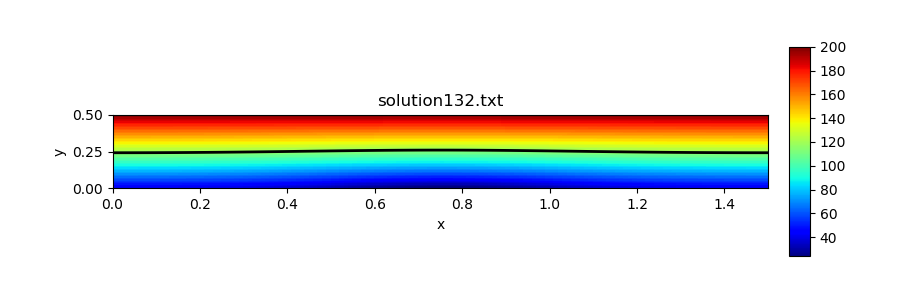
\includegraphics[width=0.75\textwidth]{solution132}
\caption{The solution along the domain at the 132nd iteration. The average temperature iso-line is drawn in black. }
\label{sol}
\end{figure}
We can also get a video of the solution using the provided \texttt{bonus.py} script which has the syntax \texttt{python3 bonus.py [input file] [solution prefix]}. An example is shown below:
\begin{verbatim}
$ python3 bonus.py input1.txt solution
file: solution000.txt, average temp: 5.521208154785093
file: solution010.txt, average temp: 26.71285983378782
file: solution020.txt, average temp: 43.33173597065316
file: solution030.txt, average temp: 59.75282142319179
file: solution040.txt, average temp: 82.22304735748604
file: solution050.txt, average temp: 97.59372842487988
file: solution060.txt, average temp: 110.10907276977017
file: solution070.txt, average temp: 116.27863777431502
file: solution080.txt, average temp: 116.28282478898845
file: solution090.txt, average temp: 116.28504182573693
file: solution100.txt, average temp: 116.2860486560187
file: solution110.txt, average temp: 116.28645882352941
file: solution120.txt, average temp: 116.28661615374627
file: solution130.txt, average temp: 116.28663556680951
file: solution132.txt, average temp: 116.28663773535905
\end{verbatim}
It also reports the files loaded and the associated average temperature reported.

\begin{rezabib}
@misc{Part1,
    author  = {CME211},
    month = {November},
    Year = {2019},
    Title = {Final Project: Part 1}
}

@misc{Part2,
    author  = {CME211},
    month = {November},
    Year = {2019},
    Title = {Final Project: Part 2}
}
\end{rezabib}
\end{document}